% =========================================================================== %

\begin{frame}[t,plain]
\titlepage
\end{frame}

% =========================================================================== %

\begin{frame}{The History of Unicode}
%
\begin{center}
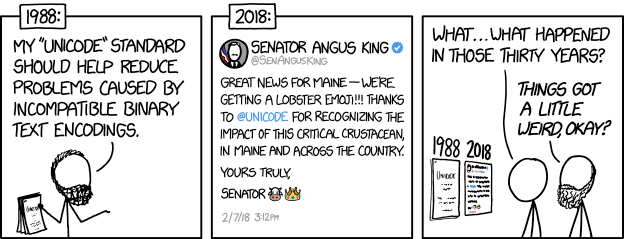
\includegraphics[width=.7\linewidth]{./gfx/xkcd-unicode-history}

\emph{2048: \enquote{Great news for Maine—we're once again an independent state!!! Thanks, @unicode, for ruling in our favor and sending troops to end New Hampshire's annexation. 
\emoji{folded-hands}\emoji{helicopter}\emoji{military-medal}}}

\vspace{6pt}
Source: \url{https://xkcd.com/1953/}

\vspace{6pt}
I spent way too much time getting LaTeX to display unicode emoji...
\end{center}
%
\end{frame}

% =========================================================================== %

\begin{frame}{The Problem}
%
\begin{columns}[t]
\column{.5\linewidth}
\begin{itemize}
\item Some characters seem never to be displayed the right way
\item Non-American characters: äöüßáèî...
\item Some sorts of interpunctation: ¿¡‽
\item Even more mundane characters like hyphens (--) or \enquote{quotation marks}
\item[\Thus] So why can't they get this right?
\end{itemize}
%
\column{.5\linewidth}
\begin{center}
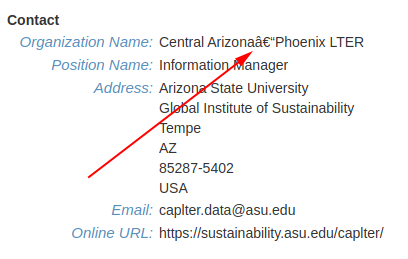
\includegraphics[width=\linewidth]{./gfx/unicode-fail} 
\end{center}
\end{columns}
%
\end{frame}

% =========================================================================== %

\begin{frame}{A Little Bit of History}
%
\begin{columns}
\column{.5\linewidth}
\begin{itemize}
\item Disk space used to be \emph{precious}
\item They had to save every single Byte
	\begin{itemize}
	\item[\thus] Cryptic commands in older languages, \eg \texttt{malloc}, \texttt{rm}, ...
	\end{itemize}
\item Down to the level of \emph{defining the format} of characters
\item One Byte (8 bit) -- one character
\item[\Thus] $2^8 = 256$ possible characters
\end{itemize}

{\tiny Picture from \url{https://www.elektronikpraxis.vogel.de/1956-die-erste-festplatte-kommt-auf-den-markt-a-418124/}}
%
\column{.5\linewidth}
\begin{center}
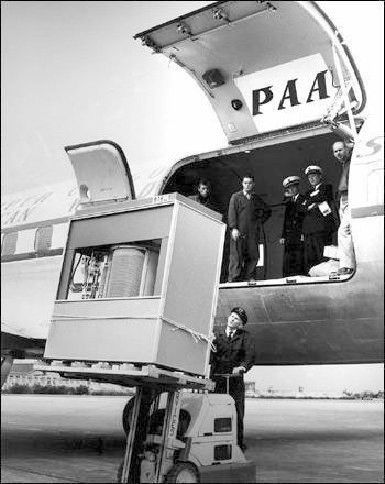
\includegraphics[width=.5\linewidth]{./gfx/IBM-305-RAMAC}

{
\scriptsize
The IBM 305 RAMAC, the first commercially available hard disk (1956) with the capacity equivalent of ca. 64.000 punch cards (a whooping 5 MB)
}
\end{center}
\end{columns}
%
\end{frame}

% =========================================================================== %

\begin{frame}{A Little Bit of History II -- Attack of the Clones}
%
\begin{columns}[t]
\column{.5\linewidth}
Humble beginnings ...
\begin{itemize}
\item Actually only 128 characters...
	\begin{itemize}
	\item Transmission over network
	\item May be faulty
	\item Introduce \emph{parity bit}: \enquote{checksum}
	\item[\Thus] 7 useable bits, $2^7 = 128$
	\end{itemize}
\item Actually only 96 characters
	\begin{itemize}
	\item First 32 characters: \enquote{non-printable}
	\item Control Characters, \eg carriage return, line feed, backspace, bell, end of file, ...
	\end{itemize}
\item[\Thus] And thus ASCII (\emph{American Standard Code for Information Interchange}) was born!
\end{itemize}
%
\column{.5\linewidth}
... but far from good enough
\begin{itemize}
\item There are are more than 96 symbols {\color{blue} \href{https://xkcd.com/285/}{[citation needed]}}
\item Only plain English texts possible
\item Soon enough: give up (replace) the parity bit mechanism to gain another 128 characters
\item[\Thus] Each nation had their own extension to ASCII ...
	\begin{itemize}
	\item {\color{blue} \href{https://en.wikipedia.org/wiki/Code_page_437}{Codepage 437}}
	\item {\color{blue} \href{https://en.wikipedia.org/wiki/Code_page_850}{Codepage 850}}
	\item {\color{blue} \href{https://en.wikipedia.org/wiki/Windows-1252}{Windows-1252}}
	\end{itemize}
\end{itemize}
\end{columns}
%
\end{frame}

% =========================================================================== %

\begin{frame}{A Little Bit of History III -- Revenge of the Sync}
%
\begin{itemize}
\item International communication only possible if \emph{character encoding} was agreed on first
\item Don't even get me started on Asia
\item Still only 224 useable characters
\item Not enough!
	\begin{itemize}
	\item Mathematical symbols
	\item Multi-language texts
	\item Arrows
	\item ...
	\end{itemize}
\item[\Thus] \emph{The world used to be a mess of home-brew solutions}
\end{itemize}
%
\end{frame}

% =========================================================================== %

\begin{frame}{A Little Bit of History IV -- A New Hope}
%
\begin{itemize}
\item October 1991: Introduction of Unicode
\item Common Standard for character encodings
	\begin{itemize}
	\item Initially: 24 scripts
	\item Current version (March 2020): 154 scripts
	\item \url{https://en.wikipedia.org/wiki/Unicode}
	\end{itemize}
\item More than a lookup table
	\begin{itemize}
	\item Maximum possible compatibility to older standards
	\item Organization into planes and blocks
	\item File size considerations
	\item Rules for composite characters
		\begin{itemize}
		\item \eg {\DejaSans y} + {\DejaSans \char"0303}  = {\DejaSans y\char"0303}
		\end{itemize}
	\end{itemize}
\item[\Thus] \emph{It took a while until the world adopted the new standard, but it solved a lot of problems!}
\item[\Thus] But: still not universally used!
\end{itemize}
%
\end{frame}

% =========================================================================== %

\begin{frame}{A Little Bit of History V -- The Encoding Strikes Back}
%
\begin{itemize}
\item 1,114,112 code points -- more than one byte necessary!
\item Expand to 4 Bytes per character?
	\begin{itemize}
	\item Quadruple file sizes and network traffic!
	\item Noticably longer CPU time
	\item Old files no longer compatible
	\end{itemize}
\item Or use only a subset of the Unicode range?
	\begin{itemize}
	\item Version 1 used only 12,795 code points -- could be done with 2 bytes per character
	\item Today: 283,506 assigned code points, still growing
	\item Old files no longer compatible
	\end{itemize}
\item Byte order?
	\begin{itemize}
	\item Little Endian or Big Endian?
	\item Byte Order Mark?
	\end{itemize}
\item[\Thus] Back to the chaos of the olden days...
\end{itemize}
%
\end{frame}

% =========================================================================== %\\

\begin{frame}{A Little Bit of History VI -- Return of the Unity}
%
\begin{columns}
\column{.5\linewidth}
\begin{itemize}
\item 1992: Presentation of UTF-8
	\begin{itemize}
	\item Unicode Transformation Format -- 8-bit.
	\end{itemize}
\item \emph{Variable} width encoding
	\begin{itemize}
	\item Compatible with ASCII
	\item Uses only as many bytes as necessary
	\item Can encode the full Unicode range
	\item Nifty extra features
	\end{itemize}
\item Finally makes up approximately 95\% of the world wide web
\item Still, some other systems in use
	\begin{itemize}
	\item ASCII/ANSI documents
	\item UTF-16, UTF-32
	\item BOMs
	\item LE/BE versions
	\end{itemize}
\end{itemize}
%
\column{.5\linewidth}
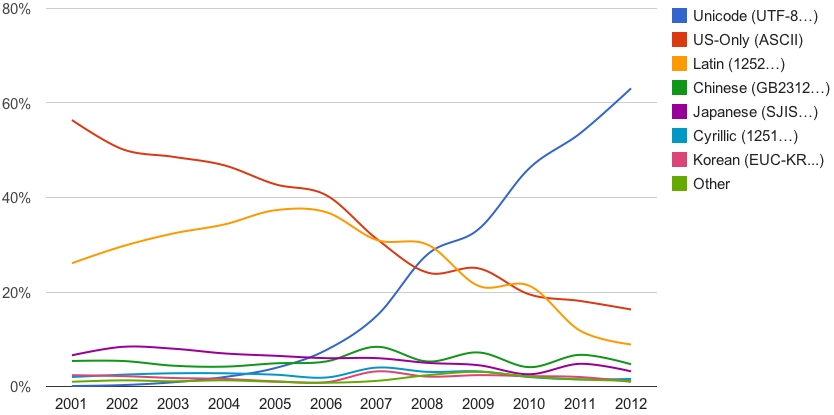
\includegraphics[width=\linewidth]{./gfx/UTF-8-website-use-2001-2012}\\
{\tiny \url{http://pinyin.info/news/2015/utf-8-unicode-vs-other-encodings-over-time/}}
\begin{itemize}
\item[\Thus] It only took 30 years in the making...
\end{itemize}
\end{columns}
%
\end{frame}

% =========================================================================== %

\begin{frame}{UTF-8: How does it work}
%
\begin{itemize}
\item Start from the \emph{code point} of your character, represent it as a binary integer
	\begin{itemize}
	\item[\Thus] {\DejaSans\char"222B} \thus 0x222B \thus\xspace {\color{purple} 10 0010 0010 1011}
	\end{itemize}
\item Count the number of bits necessary
	\begin{itemize}
	\item[\Thus] {\DejaSans\char"222B} \thus 14 bits
	\end{itemize}
\item If less than 8 bits: put all into one byte with one leading zero
	\begin{itemize}
	\item[\Thus] A \thus 0x41 \thus 100 0001 \thus\xspace {\color{orange}0}{\color{purple} 100 0001}
	\item[\Thus] ASCII compatibility
	\end{itemize}
\item If more than 8 bits: distribute over multiple bytes
	\begin{itemize}
	\item Groups of 6 bits
	\item Cap them with bits \texttt{10}
	\item Remaining bits into highest order byte with \emph{as many ones as bytes in the sequence and a zero}
	\item[\Thus] {\DejaSans\char"222B} \thus\xspace 
		{\color{orange} 1110} {\color{purple} 1000}
		{\color{orange} 10}   {\color{purple} 00 1000}
		{\color{orange} 10}   {\color{purple} 10 1011}
	\end{itemize}
\end{itemize}
%
\end{frame}

% =========================================================================== %\\

\begin{frame}{UTF-8: Why so complicated}
%
\begin{itemize}
\item Compatibility with ASCII (and therefore most ASCII-extended texts)
\item Mostly same file size for all text documents
\item Stream correction: missing bytes can easily be detected
\item Skipt to next character reasonably easy without need for extra size byte
\item[\Thus] \emph{A piece of engineering art!}
\item[\Thus] (that got used to send {\color{blue} \href{https://xkcd.com/1813/}{emoji}})
\end{itemize}
%
\end{frame}

% =========================================================================== %

\begin{frame}[fragile]{UTF-8: How to use it}
%
\begin{columns}
\column{.5\linewidth}
\begin{itemize}
\item Python: pretty much by default
	\begin{itemize}
	\item Class \inPy{str} supports multiple encodings, UTF-8 is default
	\item \inPy{help(str.encode)}
	\item Same for files -- \inPy{open} in text mode supports optional parameter encoding
	\item Behaviour plattform dependent, but usually defaults to UTF-8
	\end{itemize}
\item Files in general: set manually
	\begin{itemize}
	\item Sometimes: extra menu in editors
	\item Almost always: part of the \emph{Save As} dialog
	\end{itemize}
\item UCS: limited version of UTF-16, used with Java
\end{itemize}
%
\column{.5\linewidth}
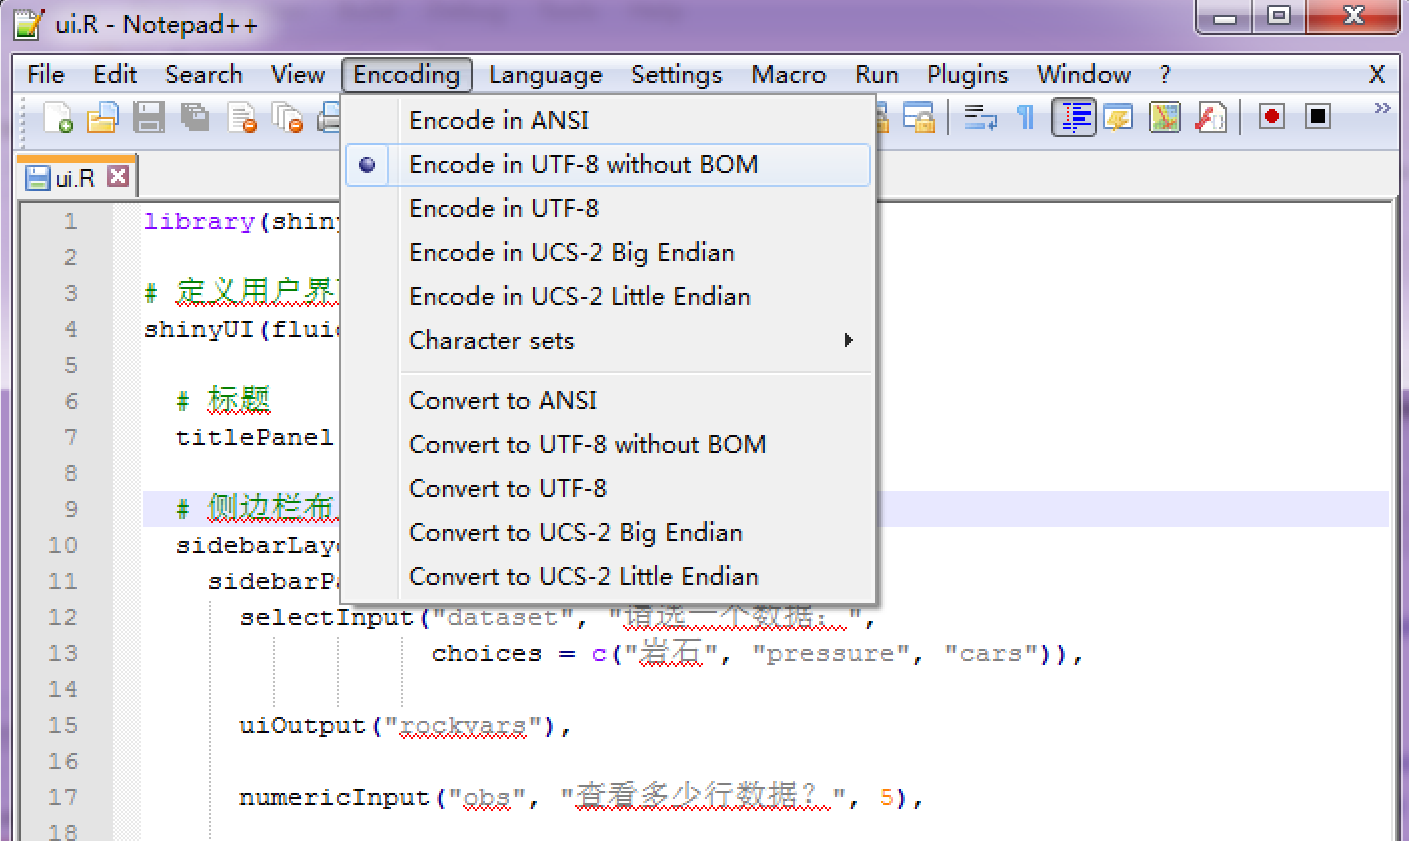
\includegraphics[width=\linewidth]{./gfx/notepad-plus-utf8.png}

\begin{itemize}
\item BOM: Byte Order Mark, special character that identifies text as Little or Big Endian
\end{itemize}
\end{columns}
%
\end{frame}

% =========================================================================== %

\begin{frame}[fragile]{Combining Diacritics and Normalization}
%
\begin{itemize}
\item Letters like Ä: common in European languages
	\begin{itemize}
	\item 8 bit encodings: unique codepoint
	\end{itemize}
\item Characters like {\DejaSans y\char"0303\char"0304\char"0305\char"0306}: less common, but possibly desired by \emph{someone}
	\begin{itemize}
	\item Actually a combination of a base character and \emph{modifiers}
	\item Same mechanism for many {\color{blue} \href{https://xkcd.com/1813/}{emoji}}: base emoji character and skin tone modifier
	\item flag emoji and nation modifier
	\end{itemize}
\item[\Thus] Desire for codepoint-compatibility at odds with logic of Unicode
\item[\Thus] They actually included both...
\item Multiple (sometimes > 2) arrangements of bytes to get the same glyph
\item[\Thus] {\color{blue} \href{https://unicode.org/reports/tr15/}{\emph{Normalization}}}: set of rules how characters \emph{should} be encoded
\item[\Thus] String parsing is a mess! Whenever possible, use pre-built libraries (\ie Python's built-in unicode handling capabilities)
\end{itemize}
%
\end{frame}

% =========================================================================== %

\begin{frame}{Wrap-Up}
%
\begin{columns}
\column{.6\linewidth}
\begin{itemize}
\item Unicode:
	\begin{itemize}
	\item How to get from number(s) to glyphs
	\item Allows uniform international communication
	\item Still has some degrees of freedom
	\end{itemize}
\item UTF-8
	\begin{itemize}
	\item How to get from number(s) to bytes
	\item Comes with or without BOM
	\end{itemize}
\item Other encodings
	\begin{itemize}
	\item Are still out there
	\item Avoid whenever possible
	\end{itemize}
\end{itemize}
%
\begin{center}
	\footnotesize
	I'm excited about the proposal to add a \enquote{brontosaurus} emoji codepoint because it has the potential to bring together a half-dozen 
	different groups of pedantic people into a single glorious internet argument.
\end{center}
%
\column{.35\linewidth}
\begin{center}
	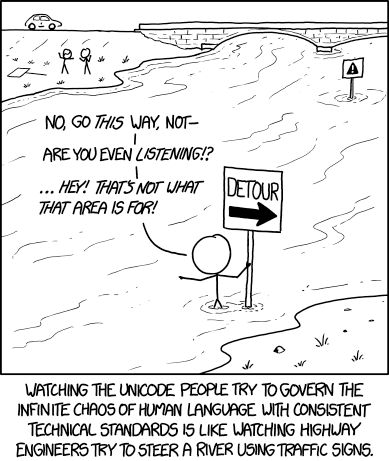
\includegraphics[width=\linewidth]{./gfx/xkcd-unicode}
	
	{\tiny
	 \texttt{https://xkcd.com/1726/}}
\end{center}
\end{columns}
%
\end{frame}